\documentclass[twoside]{book}

% Packages required by doxygen
\usepackage{calc}
\usepackage{doxygen}
\usepackage{graphicx}
\usepackage[utf8]{inputenc}
\usepackage{makeidx}
\usepackage{multicol}
\usepackage{multirow}
\usepackage{textcomp}
\usepackage[table]{xcolor}

% Font selection
\usepackage[T1]{fontenc}
\usepackage{mathptmx}
\usepackage[scaled=.90]{helvet}
\usepackage{courier}
\usepackage{amssymb}
\usepackage{sectsty}
\renewcommand{\familydefault}{\sfdefault}
\allsectionsfont{%
  \fontseries{bc}\selectfont%
  \color{darkgray}%
}
\renewcommand{\DoxyLabelFont}{%
  \fontseries{bc}\selectfont%
  \color{darkgray}%
}

% Page & text layout
\usepackage{geometry}
\geometry{%
  a4paper,%
  top=2.5cm,%
  bottom=2.5cm,%
  left=2.5cm,%
  right=2.5cm%
}
\tolerance=750
\hfuzz=15pt
\hbadness=750
\setlength{\emergencystretch}{15pt}
\setlength{\parindent}{0cm}
\setlength{\parskip}{0.2cm}
\makeatletter
\renewcommand{\paragraph}{%
  \@startsection{paragraph}{4}{0ex}{-1.0ex}{1.0ex}{%
    \normalfont\normalsize\bfseries\SS@parafont%
  }%
}
\renewcommand{\subparagraph}{%
  \@startsection{subparagraph}{5}{0ex}{-1.0ex}{1.0ex}{%
    \normalfont\normalsize\bfseries\SS@subparafont%
  }%
}
\makeatother

% Headers & footers
\usepackage{fancyhdr}
\pagestyle{fancyplain}
\fancyhead[LE]{\fancyplain{}{\bfseries\thepage}}
\fancyhead[CE]{\fancyplain{}{}}
\fancyhead[RE]{\fancyplain{}{\bfseries\leftmark}}
\fancyhead[LO]{\fancyplain{}{\bfseries\rightmark}}
\fancyhead[CO]{\fancyplain{}{}}
\fancyhead[RO]{\fancyplain{}{\bfseries\thepage}}
\fancyfoot[LE]{\fancyplain{}{}}
\fancyfoot[CE]{\fancyplain{}{}}
\fancyfoot[RE]{\fancyplain{}{\bfseries\scriptsize Generated on Wed Feb 18 2015 19\-:51\-:41 for My Project by Doxygen }}
\fancyfoot[LO]{\fancyplain{}{\bfseries\scriptsize Generated on Wed Feb 18 2015 19\-:51\-:41 for My Project by Doxygen }}
\fancyfoot[CO]{\fancyplain{}{}}
\fancyfoot[RO]{\fancyplain{}{}}
\renewcommand{\footrulewidth}{0.4pt}
\renewcommand{\chaptermark}[1]{%
  \markboth{#1}{}%
}
\renewcommand{\sectionmark}[1]{%
  \markright{\thesection\ #1}%
}

% Indices & bibliography
\usepackage{natbib}
\usepackage[titles]{tocloft}
\setcounter{tocdepth}{3}
\setcounter{secnumdepth}{5}
\makeindex

% Hyperlinks (required, but should be loaded last)
\usepackage{ifpdf}
\ifpdf
  \usepackage[pdftex,pagebackref=true]{hyperref}
\else
  \usepackage[ps2pdf,pagebackref=true]{hyperref}
\fi
\hypersetup{%
  colorlinks=true,%
  linkcolor=blue,%
  citecolor=blue,%
  unicode%
}

% Custom commands
\newcommand{\clearemptydoublepage}{%
  \newpage{\pagestyle{empty}\cleardoublepage}%
}


%===== C O N T E N T S =====

\begin{document}

% Titlepage & ToC
\hypersetup{pageanchor=false}
\pagenumbering{roman}
\begin{titlepage}
\vspace*{7cm}
\begin{center}%
{\Large My Project }\\
\vspace*{1cm}
{\large Generated by Doxygen 1.8.6}\\
\vspace*{0.5cm}
{\small Wed Feb 18 2015 19:51:41}\\
\end{center}
\end{titlepage}
\clearemptydoublepage
\tableofcontents
\clearemptydoublepage
\pagenumbering{arabic}
\hypersetup{pageanchor=true}

%--- Begin generated contents ---
\chapter{Mine\-Storm}
\label{md_README}
\hypertarget{md_README}{}
Mine\-Storm est un jeu dans lequel un petit vaisseau doit détruire des mines apparaissant aléatoirement à l'écran. Initialement proposé avec le Vectrex de Smith Engineering, nous vous proposons ici une version Qt-\/\-C++. 
\chapter{Hierarchical Index}
\section{Class Hierarchy}
This inheritance list is sorted roughly, but not completely, alphabetically\-:\begin{DoxyCompactList}
\item \contentsline{section}{Life}{\pageref{classLife}}{}
\item \contentsline{section}{Movable\-Object}{\pageref{classMovableObject}}{}
\begin{DoxyCompactList}
\item \contentsline{section}{Mine}{\pageref{classMine}}{}
\item \contentsline{section}{Ship\-Bullet}{\pageref{classShipBullet}}{}
\item \contentsline{section}{Space\-Ship}{\pageref{classSpaceShip}}{}
\end{DoxyCompactList}
\item Q\-Main\-Window\begin{DoxyCompactList}
\item \contentsline{section}{Main\-Window}{\pageref{classMainWindow}}{}
\end{DoxyCompactList}
\item Q\-Object\begin{DoxyCompactList}
\item \contentsline{section}{Game}{\pageref{classGame}}{}
\begin{DoxyCompactList}
\item \contentsline{section}{Mine\-Storm\-Game}{\pageref{classMineStormGame}}{}
\end{DoxyCompactList}
\end{DoxyCompactList}
\item Q\-Widget\begin{DoxyCompactList}
\item \contentsline{section}{Game\-Board}{\pageref{classGameBoard}}{}
\item \contentsline{section}{Overlay\-Text}{\pageref{classOverlayText}}{}
\item \contentsline{section}{Score\-Controller}{\pageref{classScoreController}}{}
\end{DoxyCompactList}
\end{DoxyCompactList}

\chapter{Class Index}
\section{Class List}
Here are the classes, structs, unions and interfaces with brief descriptions\-:\begin{DoxyCompactList}
\item\contentsline{section}{\hyperlink{classGame}{Game} \\*La classe \hyperlink{classGame}{Game} est une classe abstraite représentant base d'un jeu. Elle fournit les services de base pour controler un jeu \-: }{\pageref{classGame}}{}
\item\contentsline{section}{\hyperlink{classGameBoard}{Game\-Board} \\*La class \hyperlink{classGameBoard}{Game\-Board} définit un widget permettant l'affichage du jeu. Elle gère également les évènements clavier }{\pageref{classGameBoard}}{}
\item\contentsline{section}{\hyperlink{classLife}{Life} \\*Classe affichant les vies restantes }{\pageref{classLife}}{}
\item\contentsline{section}{\hyperlink{classMainWindow}{Main\-Window} \\*La classe \hyperlink{classMainWindow}{Main\-Window} crée un widget contenant un controller et un gameboard pour le game donné }{\pageref{classMainWindow}}{}
\item\contentsline{section}{\hyperlink{classMine}{Mine} }{\pageref{classMine}}{}
\item\contentsline{section}{\hyperlink{classMineStormGame}{Mine\-Storm\-Game} }{\pageref{classMineStormGame}}{}
\item\contentsline{section}{\hyperlink{classMovableObject}{Movable\-Object} }{\pageref{classMovableObject}}{}
\item\contentsline{section}{\hyperlink{classOverlayText}{Overlay\-Text} \\*La class \hyperlink{classOverlayText}{Overlay\-Text} définit un widget permettant l'affichage de texte par dessus l'écran de jeu comme \char`\"{}\-Pause\char`\"{} ou \char`\"{}\-Game Over\char`\"{} }{\pageref{classOverlayText}}{}
\item\contentsline{section}{\hyperlink{classScoreController}{Score\-Controller} }{\pageref{classScoreController}}{}
\item\contentsline{section}{\hyperlink{classShipBullet}{Ship\-Bullet} }{\pageref{classShipBullet}}{}
\item\contentsline{section}{\hyperlink{classSpaceShip}{Space\-Ship} }{\pageref{classSpaceShip}}{}
\end{DoxyCompactList}

\chapter{Class Documentation}
\hypertarget{classGame}{\section{Game Class Reference}
\label{classGame}\index{Game@{Game}}
}


La classe \hyperlink{classGame}{Game} est une classe abstraite représentant base d'un jeu. Elle fournit les services de base pour controler un jeu \-:  




{\ttfamily \#include $<$game.\-h$>$}

Inheritance diagram for Game\-:\begin{figure}[H]
\begin{center}
\leavevmode
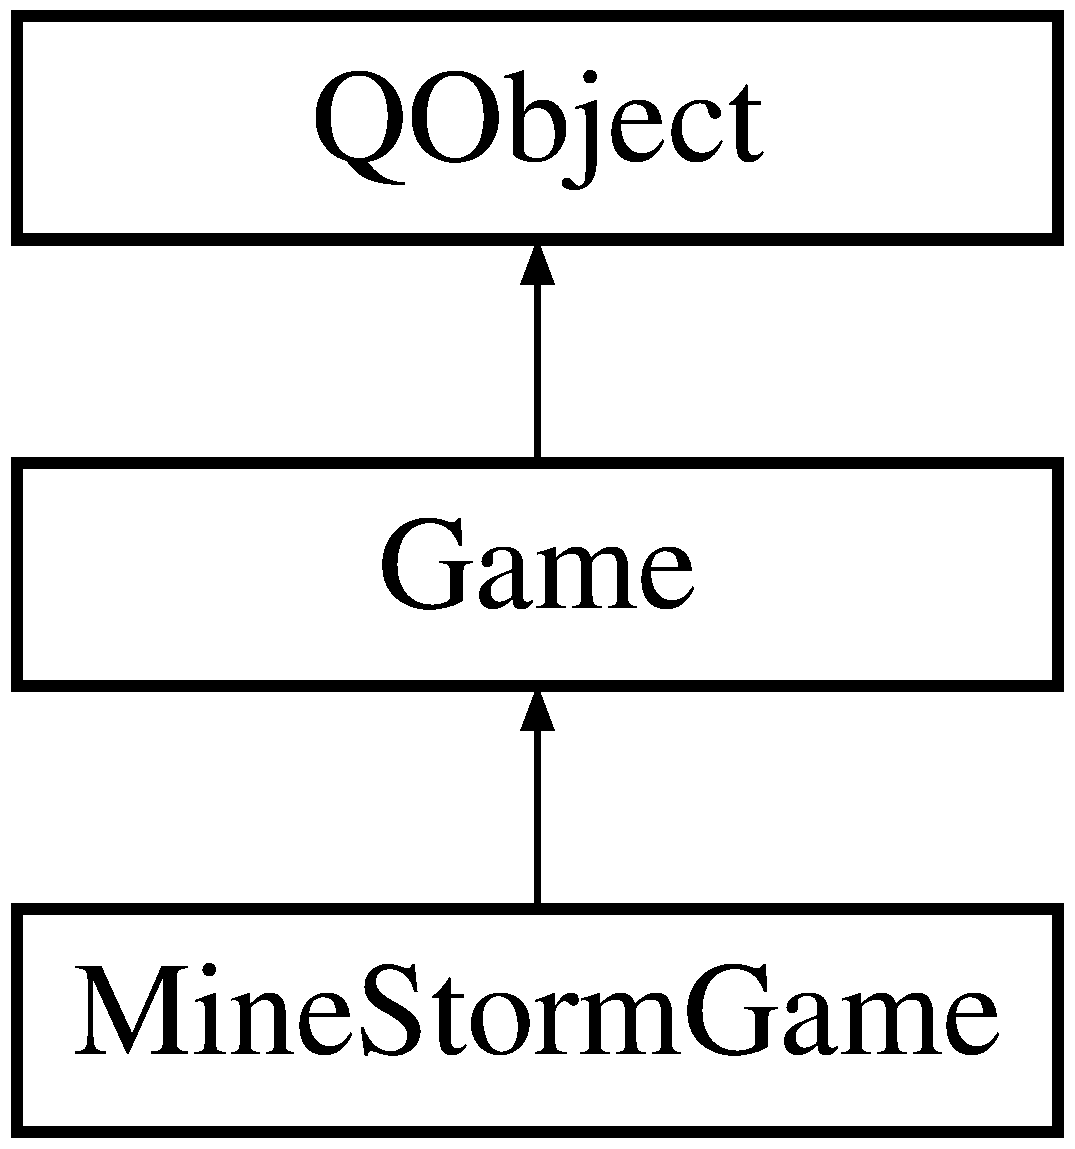
\includegraphics[height=3.000000cm]{classGame}
\end{center}
\end{figure}
\subsection*{Signals}
\begin{DoxyCompactItemize}
\item 
\hypertarget{classGame_aa56256a804a59c9031e6eb1fd9e70dc7}{void {\bfseries changed} ()}\label{classGame_aa56256a804a59c9031e6eb1fd9e70dc7}

\end{DoxyCompactItemize}
\subsection*{Public Member Functions}
\begin{DoxyCompactItemize}
\item 
\hyperlink{classGame_a76646df3c285c17da275919046f3724b}{Game} (const Q\-Size \&\hyperlink{classGame_aef028fef77b6498c42f347400b1ebf55}{size}, Q\-Object $\ast$parent)
\begin{DoxyCompactList}\small\item\em \hyperlink{classGame}{Game} contruit un jeu. \end{DoxyCompactList}\item 
\hypertarget{classGame_a3d9b98f7c4a96ecf578f75b96c9f0e90}{void \hyperlink{classGame_a3d9b98f7c4a96ecf578f75b96c9f0e90}{start} ()}\label{classGame_a3d9b98f7c4a96ecf578f75b96c9f0e90}

\begin{DoxyCompactList}\small\item\em start démarre le jeu \end{DoxyCompactList}\item 
\hypertarget{classGame_a4b507ab6c09910b3a621cf1980d65604}{void \hyperlink{classGame_a4b507ab6c09910b3a621cf1980d65604}{pause} ()}\label{classGame_a4b507ab6c09910b3a621cf1980d65604}

\begin{DoxyCompactList}\small\item\em pause met le jeu en pause \end{DoxyCompactList}\item 
\hypertarget{classGame_a39bb2fd26b5ea6b164f28f9f6723582e}{void \hyperlink{classGame_a39bb2fd26b5ea6b164f28f9f6723582e}{reset} ()}\label{classGame_a39bb2fd26b5ea6b164f28f9f6723582e}

\begin{DoxyCompactList}\small\item\em reset stop le jeu et le réinitialise \end{DoxyCompactList}\item 
\hypertarget{classGame_aff506ba208bd7428426e955e79bf3edb}{int {\bfseries get\-Score} () const }\label{classGame_aff506ba208bd7428426e955e79bf3edb}

\item 
\hypertarget{classGame_a9939ead6888ef512af8cace4a211b7b5}{void {\bfseries set\-Score} (int score)}\label{classGame_a9939ead6888ef512af8cace4a211b7b5}

\item 
const Q\-Size \& \hyperlink{classGame_aef028fef77b6498c42f347400b1ebf55}{size} () const 
\begin{DoxyCompactList}\small\item\em size retourne la taille du jeu \end{DoxyCompactList}\item 
virtual void \hyperlink{classGame_abac442d78efd636de9ab80f28eab92ef}{draw} (Q\-Painter \&painter)=0
\begin{DoxyCompactList}\small\item\em draw appelée pour afficher le jeu. Cette méthode doit être implémentée par les classes dérivées \end{DoxyCompactList}\item 
virtual void \hyperlink{classGame_a90bb392d6ca1dd209388bf43a25ac0b2}{key\-Pressed} (int key)=0
\begin{DoxyCompactList}\small\item\em key\-Pressed appélée quand l'utilisateur presse une touche \end{DoxyCompactList}\item 
virtual void \hyperlink{classGame_adad85a1736ff369687f77695fecb8ffe}{key\-Released} (int key)=0
\begin{DoxyCompactList}\small\item\em key\-Released appélée quand l'utilisateur relache une touche \end{DoxyCompactList}\item 
bool \hyperlink{classGame_abb31098c8d016b98888fe9acac497fcb}{is\-Running} () const 
\begin{DoxyCompactList}\small\item\em is\-Running retourne true si le jeu est lancé \end{DoxyCompactList}\item 
\hypertarget{classGame_a63813e2be95eae3b03483c2918558fc7}{bool {\bfseries started} () const }\label{classGame_a63813e2be95eae3b03483c2918558fc7}

\item 
\hypertarget{classGame_a7fc0fd3e81b2425bb66d52453eda86e1}{bool {\bfseries is\-Over} () const }\label{classGame_a7fc0fd3e81b2425bb66d52453eda86e1}

\end{DoxyCompactItemize}
\subsection*{Protected Member Functions}
\begin{DoxyCompactItemize}
\item 
\hypertarget{classGame_a948ffd91069e102438caeb687e1be9be}{virtual void \hyperlink{classGame_a948ffd91069e102438caeb687e1be9be}{initialize} ()=0}\label{classGame_a948ffd91069e102438caeb687e1be9be}

\begin{DoxyCompactList}\small\item\em initialize initialise ou réinitialise le jeu \end{DoxyCompactList}\end{DoxyCompactItemize}
\subsection*{Protected Attributes}
\begin{DoxyCompactItemize}
\item 
\hypertarget{classGame_a82cbb333223a3f58c565743505d73cef}{int {\bfseries \-\_\-score}}\label{classGame_a82cbb333223a3f58c565743505d73cef}

\item 
\hypertarget{classGame_a6572aacd9897d20cc1bf61c58ff49e9a}{bool {\bfseries \-\_\-game\-Over}}\label{classGame_a6572aacd9897d20cc1bf61c58ff49e9a}

\end{DoxyCompactItemize}


\subsection{Detailed Description}
La classe \hyperlink{classGame}{Game} est une classe abstraite représentant base d'un jeu. Elle fournit les services de base pour controler un jeu \-: 


\begin{DoxyItemize}
\item start/pause/reset
\item gestion des évènements souris
\item gestion des évènements clavier
\item gestion de l'affichage 
\end{DoxyItemize}

\subsection{Constructor \& Destructor Documentation}
\hypertarget{classGame_a76646df3c285c17da275919046f3724b}{\index{Game@{Game}!Game@{Game}}
\index{Game@{Game}!Game@{Game}}
\subsubsection[{Game}]{\setlength{\rightskip}{0pt plus 5cm}Game\-::\-Game (
\begin{DoxyParamCaption}
\item[{const Q\-Size \&}]{size, }
\item[{Q\-Object $\ast$}]{parent}
\end{DoxyParamCaption}
)}}\label{classGame_a76646df3c285c17da275919046f3724b}


\hyperlink{classGame}{Game} contruit un jeu. 


\begin{DoxyParams}{Parameters}
{\em size} & taille de la grille de jeu \\
\hline
{\em parent} & \\
\hline
\end{DoxyParams}


\subsection{Member Function Documentation}
\hypertarget{classGame_abac442d78efd636de9ab80f28eab92ef}{\index{Game@{Game}!draw@{draw}}
\index{draw@{draw}!Game@{Game}}
\subsubsection[{draw}]{\setlength{\rightskip}{0pt plus 5cm}virtual void Game\-::draw (
\begin{DoxyParamCaption}
\item[{Q\-Painter \&}]{painter}
\end{DoxyParamCaption}
)\hspace{0.3cm}{\ttfamily [pure virtual]}}}\label{classGame_abac442d78efd636de9ab80f28eab92ef}


draw appelée pour afficher le jeu. Cette méthode doit être implémentée par les classes dérivées 


\begin{DoxyParams}{Parameters}
{\em painter} & context d'affichage voir \href{http://doc.qt.io/qt-5/qpainter.html}{\tt la documentation Qt} \\
\hline
{\em size} & taille de la zone dans laquelle peindre le jeu \\
\hline
\end{DoxyParams}


Implemented in \hyperlink{classMineStormGame_ae801bdab673e8ef94a768937b489624d}{Mine\-Storm\-Game}.

\hypertarget{classGame_abb31098c8d016b98888fe9acac497fcb}{\index{Game@{Game}!is\-Running@{is\-Running}}
\index{is\-Running@{is\-Running}!Game@{Game}}
\subsubsection[{is\-Running}]{\setlength{\rightskip}{0pt plus 5cm}bool Game\-::is\-Running (
\begin{DoxyParamCaption}
{}
\end{DoxyParamCaption}
) const}}\label{classGame_abb31098c8d016b98888fe9acac497fcb}


is\-Running retourne true si le jeu est lancé 

\begin{DoxyReturn}{Returns}

\end{DoxyReturn}
\hypertarget{classGame_a90bb392d6ca1dd209388bf43a25ac0b2}{\index{Game@{Game}!key\-Pressed@{key\-Pressed}}
\index{key\-Pressed@{key\-Pressed}!Game@{Game}}
\subsubsection[{key\-Pressed}]{\setlength{\rightskip}{0pt plus 5cm}virtual void Game\-::key\-Pressed (
\begin{DoxyParamCaption}
\item[{int}]{key}
\end{DoxyParamCaption}
)\hspace{0.3cm}{\ttfamily [pure virtual]}}}\label{classGame_a90bb392d6ca1dd209388bf43a25ac0b2}


key\-Pressed appélée quand l'utilisateur presse une touche 


\begin{DoxyParams}{Parameters}
{\em key} & code de la touche. Tous les codes sont disponible dans \href{http://doc.qt.io/qt-5/qt.html#Key-enum}{\tt la documentation Qt} \\
\hline
\end{DoxyParams}


Implemented in \hyperlink{classMineStormGame_a242fd1067aad4a815fc0a8fe78a5fd58}{Mine\-Storm\-Game}.

\hypertarget{classGame_adad85a1736ff369687f77695fecb8ffe}{\index{Game@{Game}!key\-Released@{key\-Released}}
\index{key\-Released@{key\-Released}!Game@{Game}}
\subsubsection[{key\-Released}]{\setlength{\rightskip}{0pt plus 5cm}virtual void Game\-::key\-Released (
\begin{DoxyParamCaption}
\item[{int}]{key}
\end{DoxyParamCaption}
)\hspace{0.3cm}{\ttfamily [pure virtual]}}}\label{classGame_adad85a1736ff369687f77695fecb8ffe}


key\-Released appélée quand l'utilisateur relache une touche 


\begin{DoxyParams}{Parameters}
{\em key} & code de la touche. Tous les codes sont disponible dans \href{http://doc.qt.io/qt-5/qt.html#Key-enum}{\tt la documentation Qt} \\
\hline
\end{DoxyParams}


Implemented in \hyperlink{classMineStormGame_af5e32b922f1560cea7d5c45efcd2755e}{Mine\-Storm\-Game}.

\hypertarget{classGame_aef028fef77b6498c42f347400b1ebf55}{\index{Game@{Game}!size@{size}}
\index{size@{size}!Game@{Game}}
\subsubsection[{size}]{\setlength{\rightskip}{0pt plus 5cm}const Q\-Size \& Game\-::size (
\begin{DoxyParamCaption}
{}
\end{DoxyParamCaption}
) const}}\label{classGame_aef028fef77b6498c42f347400b1ebf55}


size retourne la taille du jeu 

\begin{DoxyReturn}{Returns}

\end{DoxyReturn}


The documentation for this class was generated from the following files\-:\begin{DoxyCompactItemize}
\item 
game.\-h\item 
game.\-cpp\end{DoxyCompactItemize}

\hypertarget{classGameBoard}{\section{Game\-Board Class Reference}
\label{classGameBoard}\index{Game\-Board@{Game\-Board}}
}


La class \hyperlink{classGameBoard}{Game\-Board} définit un widget permettant l'affichage du jeu. Elle gère également les évènements clavier.  




{\ttfamily \#include $<$gameboard.\-h$>$}

Inheritance diagram for Game\-Board\-:\begin{figure}[H]
\begin{center}
\leavevmode
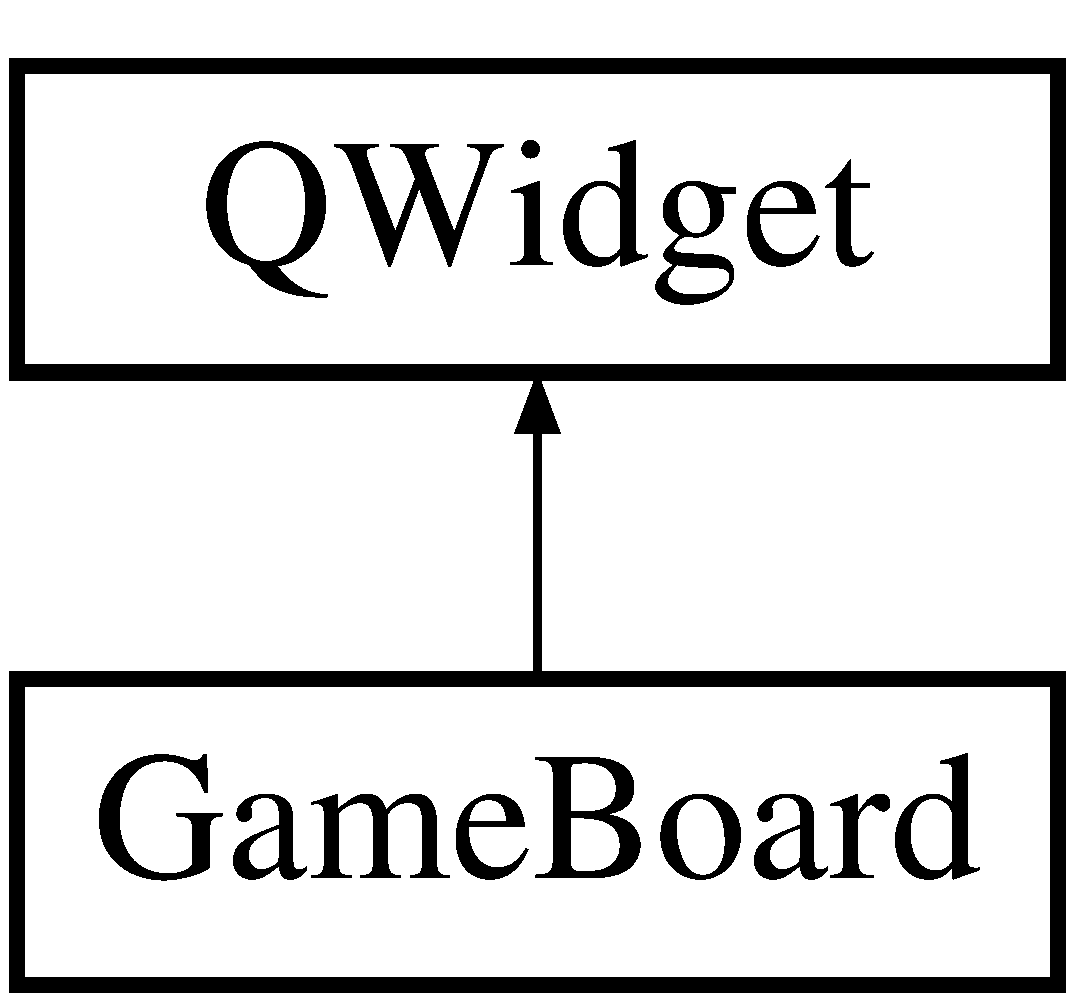
\includegraphics[height=2.000000cm]{classGameBoard}
\end{center}
\end{figure}
\subsection*{Public Member Functions}
\begin{DoxyCompactItemize}
\item 
\hypertarget{classGameBoard_a1a815e159958fed5ba4a5e23fa934835}{{\bfseries Game\-Board} (\hyperlink{classGame}{Game} $\ast$game, Q\-Widget $\ast$parent=0)}\label{classGameBoard_a1a815e159958fed5ba4a5e23fa934835}

\end{DoxyCompactItemize}
\subsection*{Protected Member Functions}
\begin{DoxyCompactItemize}
\item 
\hypertarget{classGameBoard_ae70803877f040a743eb8e424902974f3}{void {\bfseries paint\-Event} (Q\-Paint\-Event $\ast$)}\label{classGameBoard_ae70803877f040a743eb8e424902974f3}

\item 
\hypertarget{classGameBoard_a3fdf1e6bfcc24a0930196be5fc3150c1}{void {\bfseries key\-Press\-Event} (Q\-Key\-Event $\ast$event)}\label{classGameBoard_a3fdf1e6bfcc24a0930196be5fc3150c1}

\item 
\hypertarget{classGameBoard_a65228d1bdb0e856cb3115fb171185636}{void {\bfseries key\-Release\-Event} (Q\-Key\-Event $\ast$event)}\label{classGameBoard_a65228d1bdb0e856cb3115fb171185636}

\end{DoxyCompactItemize}


\subsection{Detailed Description}
La class \hyperlink{classGameBoard}{Game\-Board} définit un widget permettant l'affichage du jeu. Elle gère également les évènements clavier. 

The documentation for this class was generated from the following files\-:\begin{DoxyCompactItemize}
\item 
gameboard.\-h\item 
gameboard.\-cpp\end{DoxyCompactItemize}

\hypertarget{classLife}{\section{Life Class Reference}
\label{classLife}\index{Life@{Life}}
}


Classe affichant les vies restantes.  




{\ttfamily \#include $<$life.\-h$>$}

\subsection*{Public Member Functions}
\begin{DoxyCompactItemize}
\item 
\hyperlink{classLife_a80bafebe77f7c42607ef7b8871506b02}{Life} (Q\-Point position)
\begin{DoxyCompactList}\small\item\em Constructeur. \end{DoxyCompactList}\item 
void \hyperlink{classLife_a32e2c8f66c84246afc1f67b00486b3c9}{draw} (Q\-Painter \&painter)
\begin{DoxyCompactList}\small\item\em Classe d'affichage. \end{DoxyCompactList}\end{DoxyCompactItemize}


\subsection{Detailed Description}
Classe affichant les vies restantes. 

\subsection{Constructor \& Destructor Documentation}
\hypertarget{classLife_a80bafebe77f7c42607ef7b8871506b02}{\index{Life@{Life}!Life@{Life}}
\index{Life@{Life}!Life@{Life}}
\subsubsection[{Life}]{\setlength{\rightskip}{0pt plus 5cm}Life\-::\-Life (
\begin{DoxyParamCaption}
\item[{Q\-Point}]{position}
\end{DoxyParamCaption}
)}}\label{classLife_a80bafebe77f7c42607ef7b8871506b02}


Constructeur. 


\begin{DoxyParams}{Parameters}
{\em position} & \\
\hline
\end{DoxyParams}


\subsection{Member Function Documentation}
\hypertarget{classLife_a32e2c8f66c84246afc1f67b00486b3c9}{\index{Life@{Life}!draw@{draw}}
\index{draw@{draw}!Life@{Life}}
\subsubsection[{draw}]{\setlength{\rightskip}{0pt plus 5cm}void Life\-::draw (
\begin{DoxyParamCaption}
\item[{Q\-Painter \&}]{painter}
\end{DoxyParamCaption}
)}}\label{classLife_a32e2c8f66c84246afc1f67b00486b3c9}


Classe d'affichage. 


\begin{DoxyParams}{Parameters}
{\em painter} & \\
\hline
\end{DoxyParams}


The documentation for this class was generated from the following files\-:\begin{DoxyCompactItemize}
\item 
life.\-h\item 
life.\-cpp\end{DoxyCompactItemize}

\hypertarget{classMainWindow}{\section{Main\-Window Class Reference}
\label{classMainWindow}\index{Main\-Window@{Main\-Window}}
}


La classe \hyperlink{classMainWindow}{Main\-Window} crée un widget contenant un controller et un gameboard pour le game donné  




{\ttfamily \#include $<$mainwindow.\-h$>$}

Inheritance diagram for Main\-Window\-:\begin{figure}[H]
\begin{center}
\leavevmode
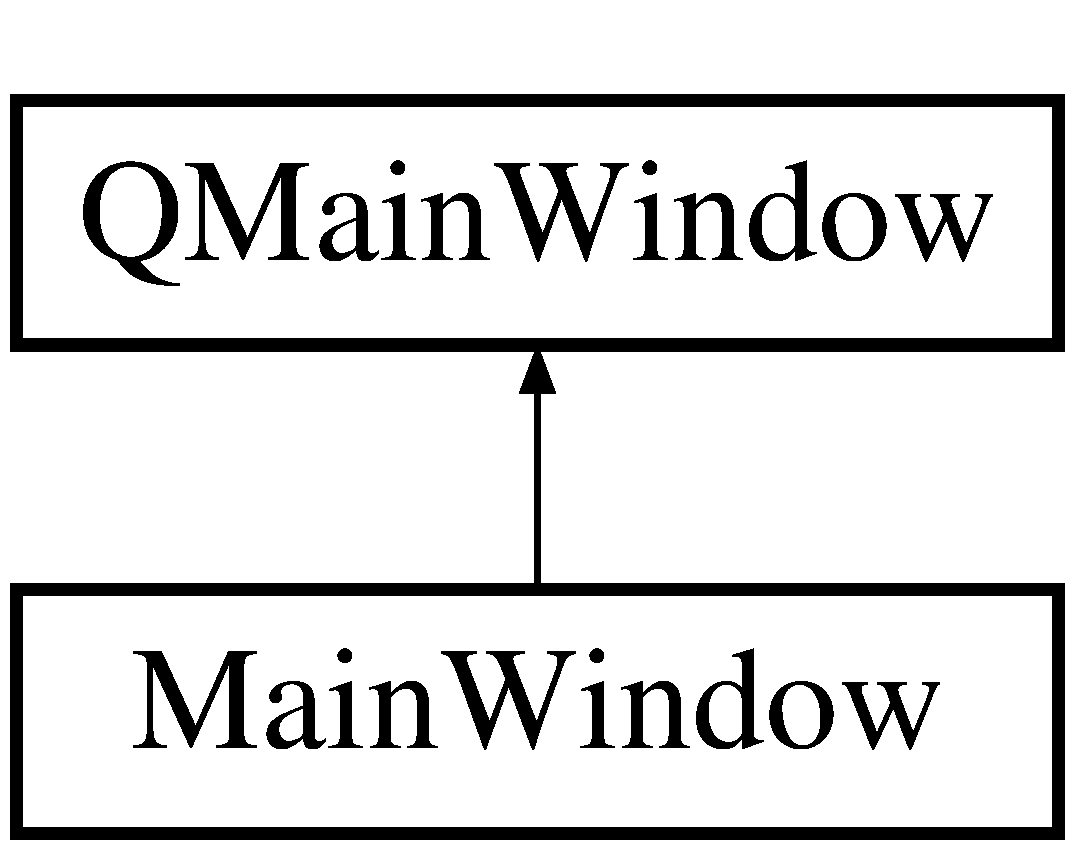
\includegraphics[height=2.000000cm]{classMainWindow}
\end{center}
\end{figure}
\subsection*{Public Member Functions}
\begin{DoxyCompactItemize}
\item 
\hypertarget{classMainWindow_a05f5d27f2bb94feb0d223c68d3ac6774}{{\bfseries Main\-Window} (\hyperlink{classGame}{Game} $\ast$game, Q\-Widget $\ast$parent=0)}\label{classMainWindow_a05f5d27f2bb94feb0d223c68d3ac6774}

\end{DoxyCompactItemize}


\subsection{Detailed Description}
La classe \hyperlink{classMainWindow}{Main\-Window} crée un widget contenant un controller et un gameboard pour le game donné 

The documentation for this class was generated from the following files\-:\begin{DoxyCompactItemize}
\item 
mainwindow.\-h\item 
mainwindow.\-cpp\end{DoxyCompactItemize}

\hypertarget{classMine}{\section{Mine Class Reference}
\label{classMine}\index{Mine@{Mine}}
}
Inheritance diagram for Mine\-:\begin{figure}[H]
\begin{center}
\leavevmode
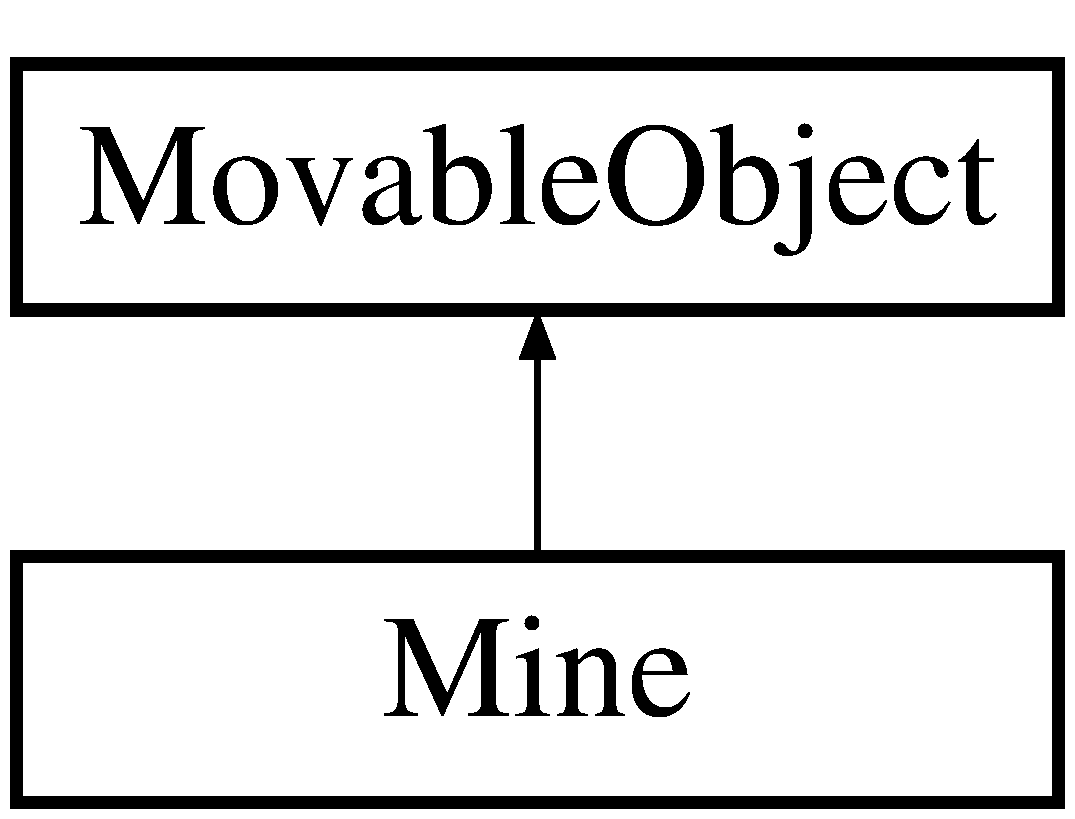
\includegraphics[height=2.000000cm]{classMine}
\end{center}
\end{figure}
\subsection*{Public Member Functions}
\begin{DoxyCompactItemize}
\item 
\hypertarget{classMine_a9d89e6260c96465e3050842bd7845778}{{\bfseries Mine} (int size, Q\-Point position, int speed, int direction)}\label{classMine_a9d89e6260c96465e3050842bd7845778}

\item 
\hypertarget{classMine_acc87edf6b5376a8e75c9673ca7414ab7}{void {\bfseries draw} (Q\-Painter \&painter)}\label{classMine_acc87edf6b5376a8e75c9673ca7414ab7}

\item 
\hypertarget{classMine_a877c2e7620c3c74d67e394e04f2ecf28}{Q\-Polygon {\bfseries get\-Polygon} () const }\label{classMine_a877c2e7620c3c74d67e394e04f2ecf28}

\item 
\hypertarget{classMine_a8adfed8ef08c5be72b3591c6cd4486db}{bool {\bfseries is\-Born} ()}\label{classMine_a8adfed8ef08c5be72b3591c6cd4486db}

\item 
\hypertarget{classMine_a0c0dc484ff8f9e36c1fa8e724b9269f8}{int {\bfseries get\-Size} ()}\label{classMine_a0c0dc484ff8f9e36c1fa8e724b9269f8}

\end{DoxyCompactItemize}
\subsection*{Additional Inherited Members}


The documentation for this class was generated from the following files\-:\begin{DoxyCompactItemize}
\item 
mine.\-h\item 
mine.\-cpp\end{DoxyCompactItemize}

\hypertarget{classMineStormGame}{\section{Mine\-Storm\-Game Class Reference}
\label{classMineStormGame}\index{Mine\-Storm\-Game@{Mine\-Storm\-Game}}
}
Inheritance diagram for Mine\-Storm\-Game\-:\begin{figure}[H]
\begin{center}
\leavevmode
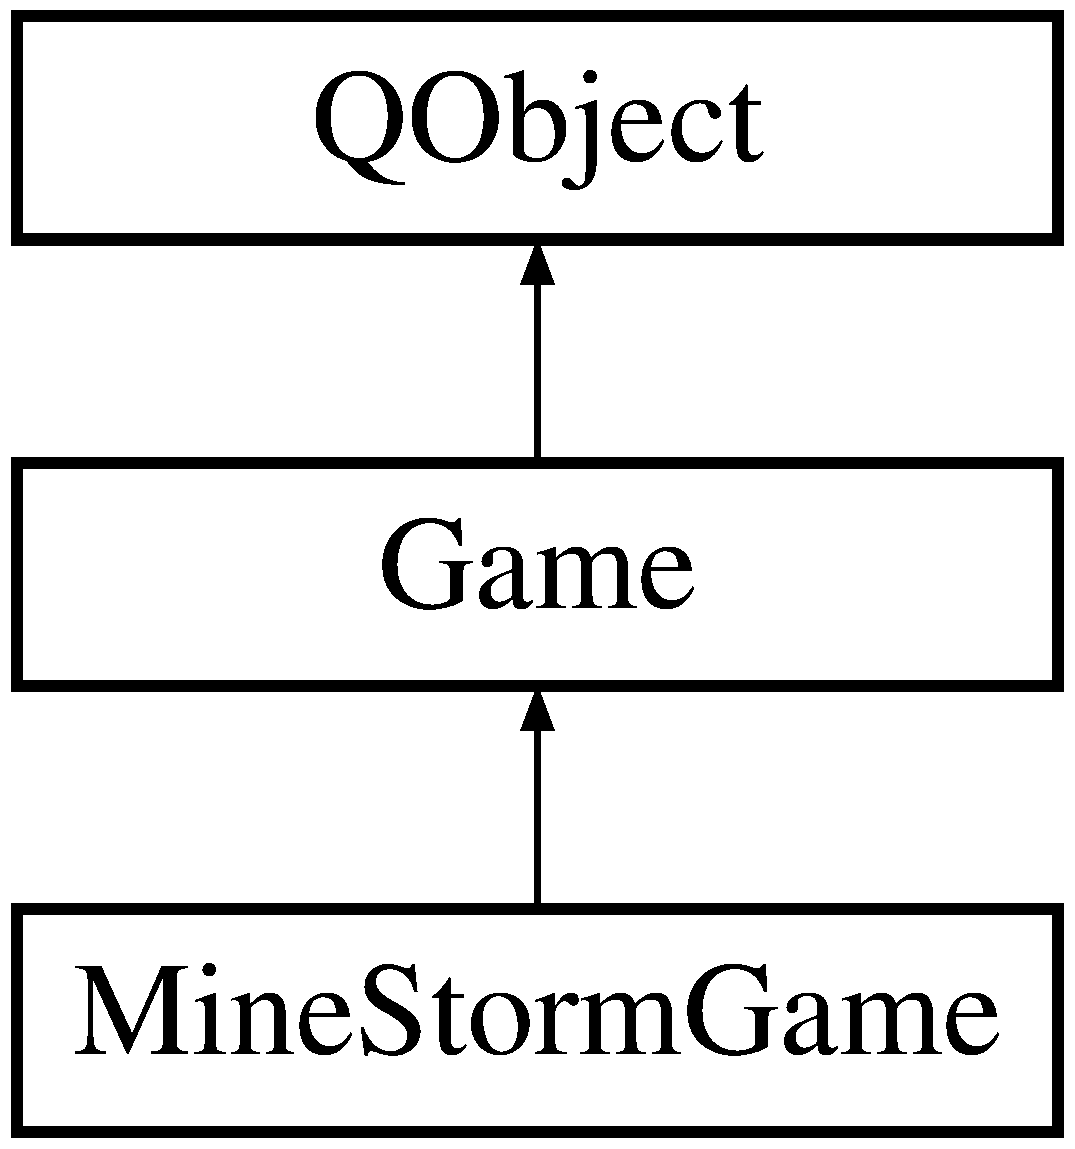
\includegraphics[height=3.000000cm]{classMineStormGame}
\end{center}
\end{figure}
\subsection*{Public Member Functions}
\begin{DoxyCompactItemize}
\item 
\hypertarget{classMineStormGame_aacea8fd6a447213810e13d6a890b67e5}{{\bfseries Mine\-Storm\-Game} (const Q\-Size \&\hyperlink{classGame_aef028fef77b6498c42f347400b1ebf55}{size}, Q\-Object $\ast$parent=nullptr)}\label{classMineStormGame_aacea8fd6a447213810e13d6a890b67e5}

\item 
virtual void \hyperlink{classMineStormGame_ae801bdab673e8ef94a768937b489624d}{draw} (Q\-Painter \&painter)
\begin{DoxyCompactList}\small\item\em draw appelée pour afficher le jeu. Cette méthode doit être implémentée par les classes dérivées \end{DoxyCompactList}\item 
void \hyperlink{classMineStormGame_a242fd1067aad4a815fc0a8fe78a5fd58}{key\-Pressed} (int key)
\begin{DoxyCompactList}\small\item\em key\-Pressed appélée quand l'utilisateur presse une touche \end{DoxyCompactList}\item 
void \hyperlink{classMineStormGame_af5e32b922f1560cea7d5c45efcd2755e}{key\-Released} (int key)
\begin{DoxyCompactList}\small\item\em key\-Released appélée quand l'utilisateur relache une touche \end{DoxyCompactList}\item 
\hypertarget{classMineStormGame_a7539c30ebd76c380b02b7a670e82e63e}{void {\bfseries generate\-Mines} (int small, int medium, int big)}\label{classMineStormGame_a7539c30ebd76c380b02b7a670e82e63e}

\item 
\hypertarget{classMineStormGame_a65140f427616478dcb7d8e8c38bb03a2}{void {\bfseries loose\-Life} ()}\label{classMineStormGame_a65140f427616478dcb7d8e8c38bb03a2}

\end{DoxyCompactItemize}
\subsection*{Additional Inherited Members}


\subsection{Member Function Documentation}
\hypertarget{classMineStormGame_ae801bdab673e8ef94a768937b489624d}{\index{Mine\-Storm\-Game@{Mine\-Storm\-Game}!draw@{draw}}
\index{draw@{draw}!MineStormGame@{Mine\-Storm\-Game}}
\subsubsection[{draw}]{\setlength{\rightskip}{0pt plus 5cm}void Mine\-Storm\-Game\-::draw (
\begin{DoxyParamCaption}
\item[{Q\-Painter \&}]{painter}
\end{DoxyParamCaption}
)\hspace{0.3cm}{\ttfamily [virtual]}}}\label{classMineStormGame_ae801bdab673e8ef94a768937b489624d}


draw appelée pour afficher le jeu. Cette méthode doit être implémentée par les classes dérivées 


\begin{DoxyParams}{Parameters}
{\em painter} & context d'affichage voir \href{http://doc.qt.io/qt-5/qpainter.html}{\tt la documentation Qt} \\
\hline
{\em size} & taille de la zone dans laquelle peindre le jeu \\
\hline
\end{DoxyParams}


Implements \hyperlink{classGame_abac442d78efd636de9ab80f28eab92ef}{Game}.

\hypertarget{classMineStormGame_a242fd1067aad4a815fc0a8fe78a5fd58}{\index{Mine\-Storm\-Game@{Mine\-Storm\-Game}!key\-Pressed@{key\-Pressed}}
\index{key\-Pressed@{key\-Pressed}!MineStormGame@{Mine\-Storm\-Game}}
\subsubsection[{key\-Pressed}]{\setlength{\rightskip}{0pt plus 5cm}void Mine\-Storm\-Game\-::key\-Pressed (
\begin{DoxyParamCaption}
\item[{int}]{key}
\end{DoxyParamCaption}
)\hspace{0.3cm}{\ttfamily [virtual]}}}\label{classMineStormGame_a242fd1067aad4a815fc0a8fe78a5fd58}


key\-Pressed appélée quand l'utilisateur presse une touche 


\begin{DoxyParams}{Parameters}
{\em key} & code de la touche. Tous les codes sont disponible dans \href{http://doc.qt.io/qt-5/qt.html#Key-enum}{\tt la documentation Qt} \\
\hline
\end{DoxyParams}


Implements \hyperlink{classGame_a90bb392d6ca1dd209388bf43a25ac0b2}{Game}.

\hypertarget{classMineStormGame_af5e32b922f1560cea7d5c45efcd2755e}{\index{Mine\-Storm\-Game@{Mine\-Storm\-Game}!key\-Released@{key\-Released}}
\index{key\-Released@{key\-Released}!MineStormGame@{Mine\-Storm\-Game}}
\subsubsection[{key\-Released}]{\setlength{\rightskip}{0pt plus 5cm}void Mine\-Storm\-Game\-::key\-Released (
\begin{DoxyParamCaption}
\item[{int}]{key}
\end{DoxyParamCaption}
)\hspace{0.3cm}{\ttfamily [virtual]}}}\label{classMineStormGame_af5e32b922f1560cea7d5c45efcd2755e}


key\-Released appélée quand l'utilisateur relache une touche 


\begin{DoxyParams}{Parameters}
{\em key} & code de la touche. Tous les codes sont disponible dans \href{http://doc.qt.io/qt-5/qt.html#Key-enum}{\tt la documentation Qt} \\
\hline
\end{DoxyParams}


Implements \hyperlink{classGame_adad85a1736ff369687f77695fecb8ffe}{Game}.



The documentation for this class was generated from the following files\-:\begin{DoxyCompactItemize}
\item 
minestormgame.\-h\item 
minestormgame.\-cpp\end{DoxyCompactItemize}

\hypertarget{classMovableObject}{\section{Movable\-Object Class Reference}
\label{classMovableObject}\index{Movable\-Object@{Movable\-Object}}
}
Inheritance diagram for Movable\-Object\-:\begin{figure}[H]
\begin{center}
\leavevmode
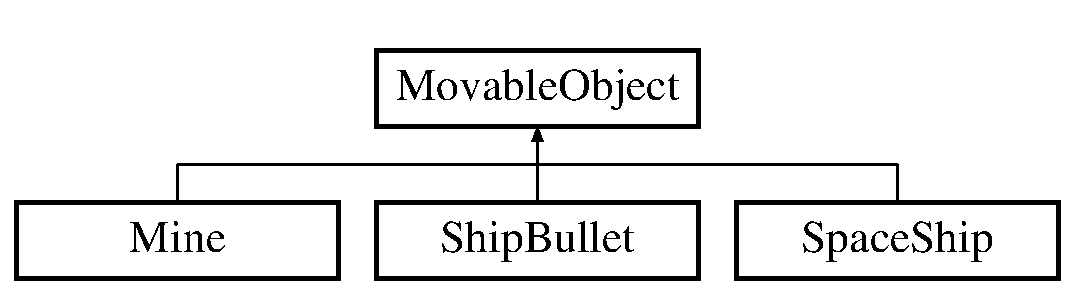
\includegraphics[height=2.000000cm]{classMovableObject}
\end{center}
\end{figure}
\subsection*{Public Member Functions}
\begin{DoxyCompactItemize}
\item 
\hypertarget{classMovableObject_a9b2b8fc00404965484a7885fd207da24}{{\bfseries Movable\-Object} (Q\-Point position=Q\-Point(120, 120), int speed=0, int direction=0)}\label{classMovableObject_a9b2b8fc00404965484a7885fd207da24}

\item 
\hypertarget{classMovableObject_a7112d6aedca3f9e2a2cfa3d6735a714e}{virtual void {\bfseries draw} (Q\-Painter \&painter)=0}\label{classMovableObject_a7112d6aedca3f9e2a2cfa3d6735a714e}

\item 
\hypertarget{classMovableObject_a574fbfa8b20e5a4d40e57346882e48b0}{Q\-Point {\bfseries get\-Position} ()}\label{classMovableObject_a574fbfa8b20e5a4d40e57346882e48b0}

\item 
\hypertarget{classMovableObject_a31182609e87fb111c14eaf95adf18530}{void {\bfseries set\-Speed} (int speed)}\label{classMovableObject_a31182609e87fb111c14eaf95adf18530}

\item 
\hypertarget{classMovableObject_a8cccf8afb9b7bfef062b24e8ecf768ad}{int {\bfseries get\-Speed} ()}\label{classMovableObject_a8cccf8afb9b7bfef062b24e8ecf768ad}

\item 
\hypertarget{classMovableObject_a98eaac3597cd98d7c0072448fceefe42}{void {\bfseries set\-Direction} (int angle)}\label{classMovableObject_a98eaac3597cd98d7c0072448fceefe42}

\item 
\hypertarget{classMovableObject_a874e1be122655380b1b0fa94e8100298}{int {\bfseries get\-Direction} ()}\label{classMovableObject_a874e1be122655380b1b0fa94e8100298}

\item 
\hypertarget{classMovableObject_a4f110e42ed00a673b7b6d9f453f75c8e}{void {\bfseries move} (Q\-Size bounds)}\label{classMovableObject_a4f110e42ed00a673b7b6d9f453f75c8e}

\item 
\hypertarget{classMovableObject_a468258e6606987d94bb56a7c193d6f23}{virtual bool {\bfseries in\-Contact} (\hyperlink{classMovableObject}{Movable\-Object} const \&object) const }\label{classMovableObject_a468258e6606987d94bb56a7c193d6f23}

\item 
\hypertarget{classMovableObject_af49dab7d8966f5cebb7adcda2f74cc25}{virtual Q\-Polygon {\bfseries get\-Polygon} () const =0}\label{classMovableObject_af49dab7d8966f5cebb7adcda2f74cc25}

\end{DoxyCompactItemize}
\subsection*{Protected Attributes}
\begin{DoxyCompactItemize}
\item 
\hypertarget{classMovableObject_a9933b4063dbd98809bf268099e714504}{Q\-Point {\bfseries \-\_\-position}}\label{classMovableObject_a9933b4063dbd98809bf268099e714504}

\item 
\hypertarget{classMovableObject_a8464b267992970b197fe83da6b1ca954}{int {\bfseries \-\_\-direction}}\label{classMovableObject_a8464b267992970b197fe83da6b1ca954}

\item 
\hypertarget{classMovableObject_a025fbf9a26bb0157c1017c996dbc32f2}{Q\-Point {\bfseries \-\_\-speed}}\label{classMovableObject_a025fbf9a26bb0157c1017c996dbc32f2}

\end{DoxyCompactItemize}


The documentation for this class was generated from the following files\-:\begin{DoxyCompactItemize}
\item 
movableobject.\-h\item 
movableobject.\-cpp\end{DoxyCompactItemize}

\hypertarget{classOverlayText}{\section{Overlay\-Text Class Reference}
\label{classOverlayText}\index{Overlay\-Text@{Overlay\-Text}}
}


La class \hyperlink{classOverlayText}{Overlay\-Text} définit un widget permettant l'affichage de texte par dessus l'écran de jeu comme \char`\"{}\-Pause\char`\"{} ou \char`\"{}\-Game Over\char`\"{}.  




{\ttfamily \#include $<$overlaytext.\-h$>$}

Inheritance diagram for Overlay\-Text\-:\begin{figure}[H]
\begin{center}
\leavevmode
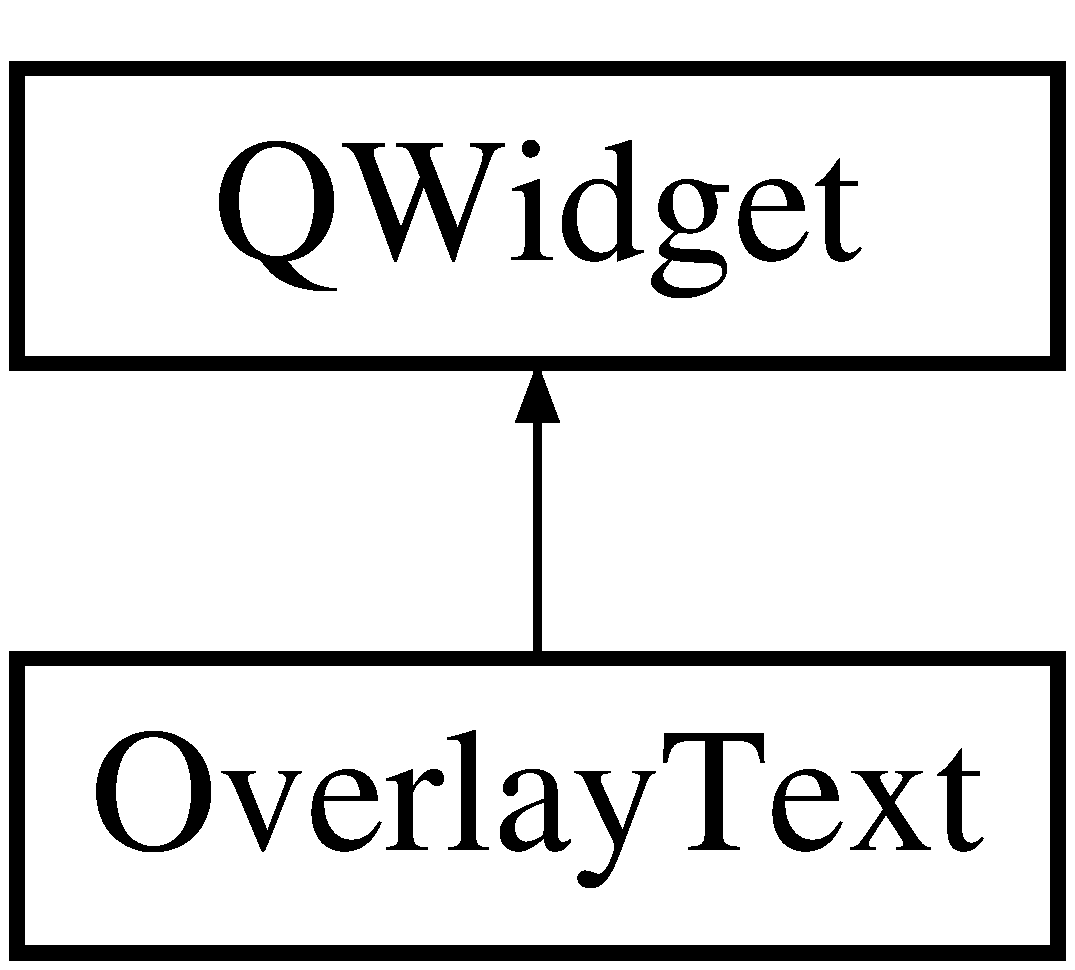
\includegraphics[height=2.000000cm]{classOverlayText}
\end{center}
\end{figure}
\subsection*{Public Member Functions}
\begin{DoxyCompactItemize}
\item 
\hypertarget{classOverlayText_a23f5d7cb173c3ea9b22756891ba055f5}{{\bfseries Overlay\-Text} (\hyperlink{classGame}{Game} $\ast$game, Q\-Widget $\ast$parent=0)}\label{classOverlayText_a23f5d7cb173c3ea9b22756891ba055f5}

\end{DoxyCompactItemize}
\subsection*{Protected Member Functions}
\begin{DoxyCompactItemize}
\item 
\hypertarget{classOverlayText_a7e395d2f1a573e7dbba3fb1676d583a1}{void {\bfseries paint\-Event} (Q\-Paint\-Event $\ast$)}\label{classOverlayText_a7e395d2f1a573e7dbba3fb1676d583a1}

\end{DoxyCompactItemize}


\subsection{Detailed Description}
La class \hyperlink{classOverlayText}{Overlay\-Text} définit un widget permettant l'affichage de texte par dessus l'écran de jeu comme \char`\"{}\-Pause\char`\"{} ou \char`\"{}\-Game Over\char`\"{}. 

The documentation for this class was generated from the following files\-:\begin{DoxyCompactItemize}
\item 
overlaytext.\-h\item 
overlaytext.\-cpp\end{DoxyCompactItemize}

\hypertarget{classScoreController}{\section{Score\-Controller Class Reference}
\label{classScoreController}\index{Score\-Controller@{Score\-Controller}}
}
Inheritance diagram for Score\-Controller\-:\begin{figure}[H]
\begin{center}
\leavevmode
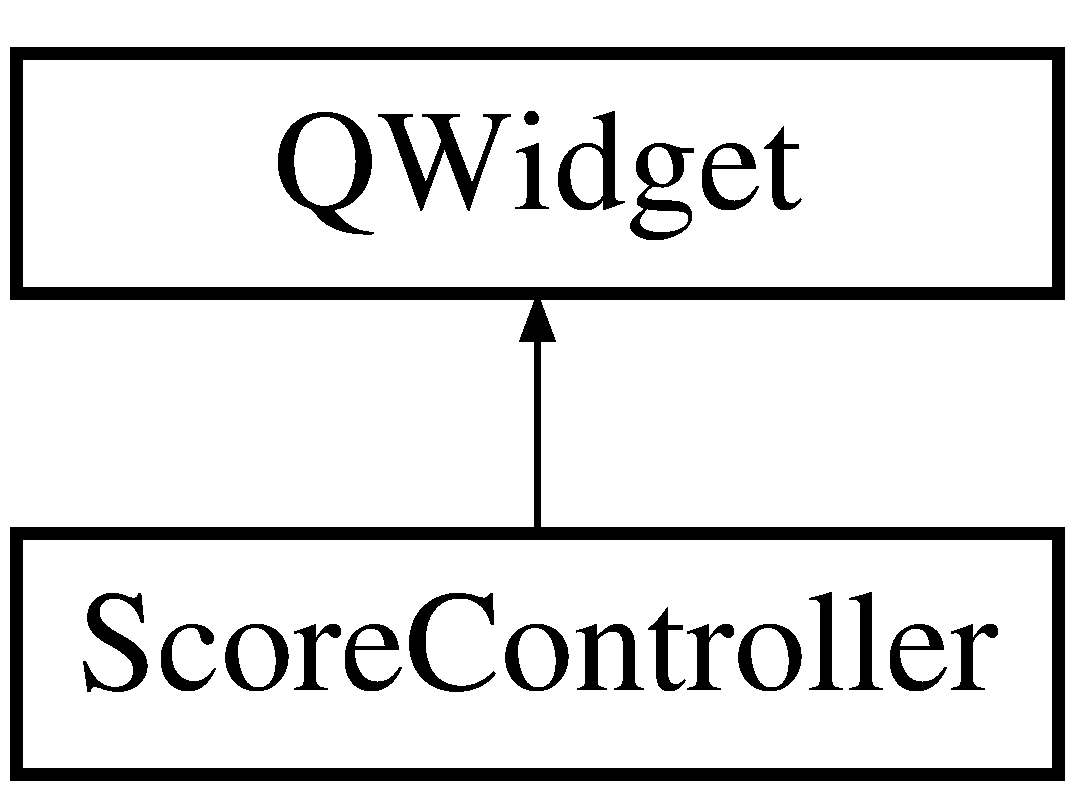
\includegraphics[height=2.000000cm]{classScoreController}
\end{center}
\end{figure}
\subsection*{Public Slots}
\begin{DoxyCompactItemize}
\item 
\hypertarget{classScoreController_a657c1dac92c56059d52cabe78ec2d7e1}{void {\bfseries refresh} ()}\label{classScoreController_a657c1dac92c56059d52cabe78ec2d7e1}

\end{DoxyCompactItemize}
\subsection*{Public Member Functions}
\begin{DoxyCompactItemize}
\item 
\hypertarget{classScoreController_a50490142b56d6d83df35c814dcff963e}{{\bfseries Score\-Controller} (\hyperlink{classGame}{Game} $\ast$game, Q\-Widget $\ast$parent=0)}\label{classScoreController_a50490142b56d6d83df35c814dcff963e}

\end{DoxyCompactItemize}


The documentation for this class was generated from the following files\-:\begin{DoxyCompactItemize}
\item 
scorecontroller.\-h\item 
scorecontroller.\-cpp\end{DoxyCompactItemize}

\hypertarget{classShipBullet}{\section{Ship\-Bullet Class Reference}
\label{classShipBullet}\index{Ship\-Bullet@{Ship\-Bullet}}
}
Inheritance diagram for Ship\-Bullet\-:\begin{figure}[H]
\begin{center}
\leavevmode
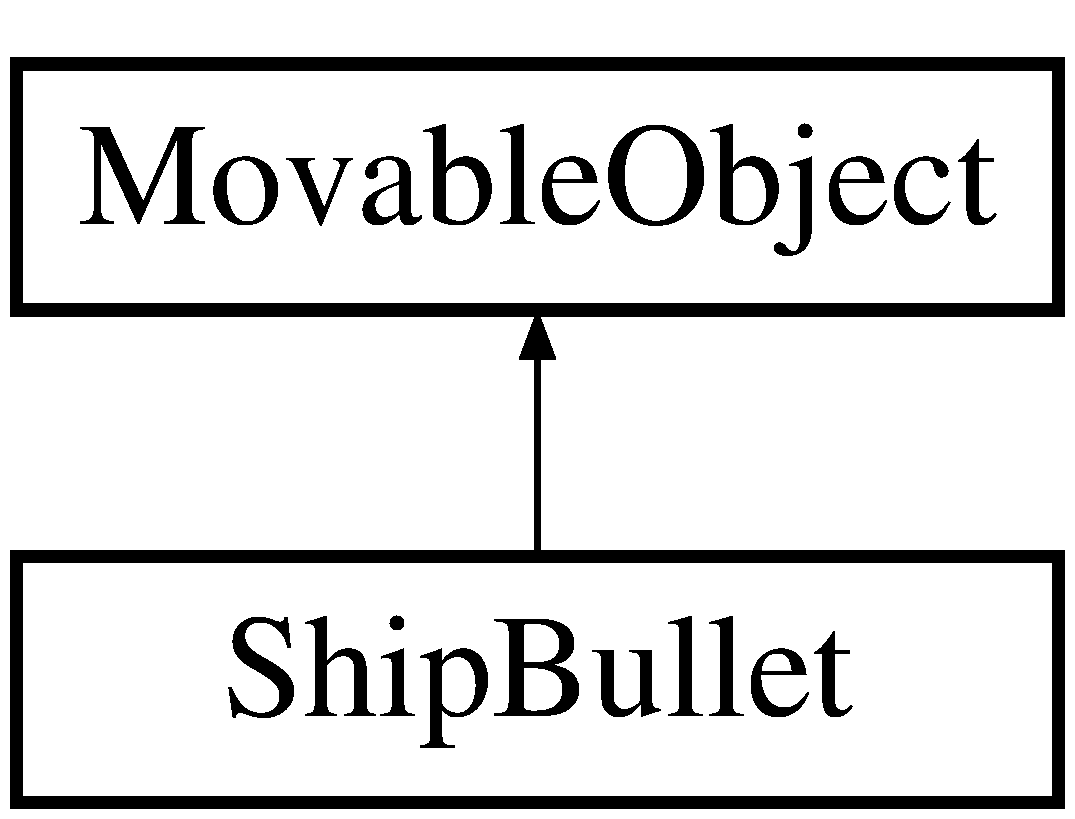
\includegraphics[height=2.000000cm]{classShipBullet}
\end{center}
\end{figure}
\subsection*{Public Member Functions}
\begin{DoxyCompactItemize}
\item 
\hypertarget{classShipBullet_a5b6665ee24ceeb4b7410786581ef885f}{{\bfseries Ship\-Bullet} (Q\-Point position, int speed, int orientation)}\label{classShipBullet_a5b6665ee24ceeb4b7410786581ef885f}

\item 
\hypertarget{classShipBullet_afb06f07a413c735cb69a1f16756d89a4}{void {\bfseries draw} (Q\-Painter \&painter)}\label{classShipBullet_afb06f07a413c735cb69a1f16756d89a4}

\item 
\hypertarget{classShipBullet_a5bf79549af9ec712e03c981cfc85bacf}{bool {\bfseries is\-Alive} ()}\label{classShipBullet_a5bf79549af9ec712e03c981cfc85bacf}

\item 
\hypertarget{classShipBullet_afe540907a92b8a833774b5ff78b71b9e}{Q\-Polygon {\bfseries get\-Polygon} () const }\label{classShipBullet_afe540907a92b8a833774b5ff78b71b9e}

\end{DoxyCompactItemize}
\subsection*{Additional Inherited Members}


The documentation for this class was generated from the following files\-:\begin{DoxyCompactItemize}
\item 
shipbullet.\-h\item 
shipbullet.\-cpp\end{DoxyCompactItemize}

\hypertarget{classSpaceShip}{\section{Space\-Ship Class Reference}
\label{classSpaceShip}\index{Space\-Ship@{Space\-Ship}}
}
Inheritance diagram for Space\-Ship\-:\begin{figure}[H]
\begin{center}
\leavevmode
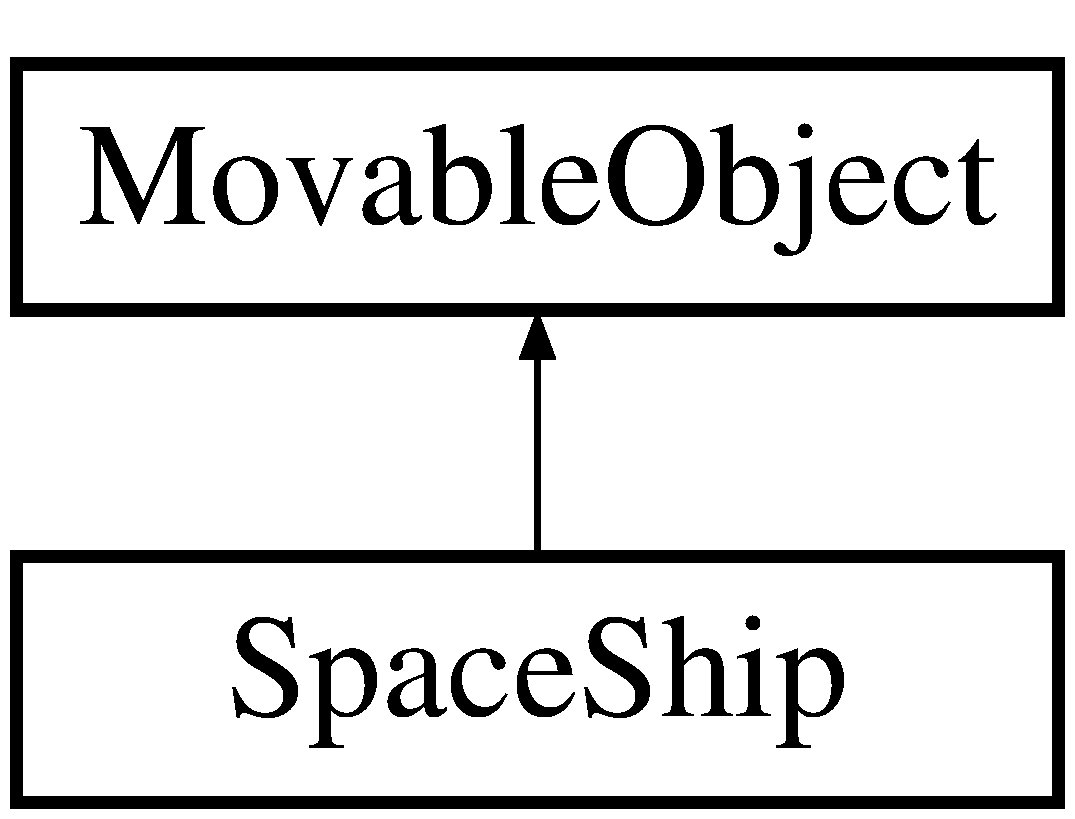
\includegraphics[height=2.000000cm]{classSpaceShip}
\end{center}
\end{figure}
\subsection*{Public Member Functions}
\begin{DoxyCompactItemize}
\item 
\hypertarget{classSpaceShip_adbc4de15943ec4e773fb4aa2c7af80d7}{{\bfseries Space\-Ship} (Q\-Point position, int orientation=180)}\label{classSpaceShip_adbc4de15943ec4e773fb4aa2c7af80d7}

\item 
\hypertarget{classSpaceShip_af818580ba0af92e9d2fc802062cb4230}{void {\bfseries draw} (Q\-Painter \&painter)}\label{classSpaceShip_af818580ba0af92e9d2fc802062cb4230}

\item 
\hypertarget{classSpaceShip_ab22ffc09f85aedf98631a95fe1dff50d}{void {\bfseries rotate\-Left} ()}\label{classSpaceShip_ab22ffc09f85aedf98631a95fe1dff50d}

\item 
\hypertarget{classSpaceShip_aaeee70ef27051a1113ce68def76f5a3e}{void {\bfseries rotate\-Right} ()}\label{classSpaceShip_aaeee70ef27051a1113ce68def76f5a3e}

\item 
\hypertarget{classSpaceShip_ace0da5ec860ed1fa8aafaa3e6c00dcdd}{void {\bfseries accelerate} ()}\label{classSpaceShip_ace0da5ec860ed1fa8aafaa3e6c00dcdd}

\item 
\hypertarget{classSpaceShip_ac1503d09ed0843352b9ac749a1614bff}{void {\bfseries stop\-Acceleration} ()}\label{classSpaceShip_ac1503d09ed0843352b9ac749a1614bff}

\item 
\hypertarget{classSpaceShip_a257ea4b0622608577d6158274b8eb7c3}{int {\bfseries get\-Orientation} ()}\label{classSpaceShip_a257ea4b0622608577d6158274b8eb7c3}

\item 
\hypertarget{classSpaceShip_a59618f15c166a31a38b9f303fa060bb1}{void {\bfseries stop} ()}\label{classSpaceShip_a59618f15c166a31a38b9f303fa060bb1}

\item 
\hypertarget{classSpaceShip_a641a7f1558eba1082b76e356923adabc}{Q\-Polygon {\bfseries get\-Polygon} () const }\label{classSpaceShip_a641a7f1558eba1082b76e356923adabc}

\item 
\hypertarget{classSpaceShip_ad0a5b483b3da04c809364b0ff6fbb2da}{bool {\bfseries is\-Invincible} ()}\label{classSpaceShip_ad0a5b483b3da04c809364b0ff6fbb2da}

\item 
\hypertarget{classSpaceShip_ad16e8b430cd9fe8a7c81e6f167986c58}{void {\bfseries reset\-God\-Mode} ()}\label{classSpaceShip_ad16e8b430cd9fe8a7c81e6f167986c58}

\end{DoxyCompactItemize}
\subsection*{Additional Inherited Members}


The documentation for this class was generated from the following files\-:\begin{DoxyCompactItemize}
\item 
spaceship.\-h\item 
spaceship.\-cpp\end{DoxyCompactItemize}

%--- End generated contents ---

% Index
\newpage
\phantomsection
\addcontentsline{toc}{chapter}{Index}
\printindex

\end{document}
